\documentclass[11pt]{article}
% Кодировка и язык
\usepackage[utf8]{inputenc}           % Кодировка исходного файла (UTF-8)
\usepackage[T2A]{fontenc}             % Кодировка шрифтов для кириллицы
\usepackage[english,russian]{babel}   % Локализация: русские названия, переносы

% Поиск в PDF
\usepackage{cmap}                     

% Поля страницы
\usepackage{geometry}
\geometry{left=2cm, right=2cm, top=2cm, bottom=2cm}

% Математика
\usepackage{amsmath, amssymb, amsthm} % Базовые пакеты для математики
\usepackage{mathtools}                % Расширение amsmath (доп. символы и окружения)

% Картинки
\usepackage{graphicx}                 % Вставка картинок (\includegraphics)
\graphicspath{{pictures/}}            % Путь к папке с картинками
\usepackage{float}                    % Позволяет использовать [H] для жёсткого позиционирования
\usepackage{wrapfig}                  % Обтекание текста вокруг картинок

% Таблицы
\usepackage{array}                    % Расширенные возможности для таблиц
\usepackage{booktabs}                 % Красивые таблицы (\toprule, \midrule, \bottomrule)
\usepackage{multirow}                 % Объединение строк в таблицах
\usepackage{tabularx}                 % Таблицы с автоматической шириной колонок
\usepackage{ragged2e}                 % Улучшенное выравнивание (используется в tabularx)

% Списки
\usepackage{enumitem}                 % Гибкая настройка списков (itemize, enumerate)

% Колонтитулы
\usepackage{fancyhdr}                 

% Гиперссылки
\usepackage{xcolor}                   % Работа с цветами
\usepackage{hyperref}                 % Гиперссылки, оглавление, перекрёстные ссылки

% Умные ссылки
\usepackage{cleveref}                 

% Типографика
\usepackage[expansion=false]{microtype}                % Улучшает переносы и межсловные расстояния

% Подписи к картинкам и таблицам
\usepackage{caption}                  % Настройка подписей (шрифт, отступы)

% Рисование схем и графиков
\usepackage{tikz}                     % Рисование схем, графиков, диаграмм
\usepackage{pgfplots}                 % Построение графиков функций (на основе tikz)
\pgfplotsset{compat=newest}           % Версия совместимости pgfplots

% Алгоритмы и код
\usepackage{algorithm}                % Окружения для алгоритмов
\usepackage{algorithmic}              % Синтаксис для алгоритмов
\usepackage{listings}                 % Вставка кода с подсветкой синтаксиса


% Настройка нумерации секций и подсекций
\renewcommand{\thesection}{\arabic{section}}                   
\renewcommand{\thesubsection}{\thesection.\arabic{subsection}} 


% Настройка списков: убираем лишние отступы слева
\setlist[itemize]{leftmargin=*}
\setlist[enumerate]{leftmargin=*}


% Определение окружений для теорем, лемм, определений и т.д.
% Нумерация привязана к номеру секции
\newtheorem{theorem}{Теорема}[section]
\newtheorem{definition}{Определение}[section]
\newtheorem{remark}{Замечание}[section]
\newtheorem{lemma}{Лемма}[section]
\newtheorem{example}{Пример}[section]
\newtheorem{consequence}{Следствие}[section]
\newtheorem{algorithmm}{Алгоритм}
\newtheorem{question}{Вопрос}[section]
\newtheorem{answer}{Ответ}[section]
\newtheorem{statement}{Утверждение}[section]


% Определение цветов
\definecolor{pblue}{rgb}{0.13,0.13,1}    
\definecolor{pgreen}{rgb}{0,0.5,0}       
\definecolor{pred}{rgb}{0.9,0,0}         
\definecolor{pgrey}{rgb}{0.46,0.45,0.48}

\usepackage{tikz}

\DeclareMathOperator{\SAT}{SAT}
\DeclareMathOperator{\MSAT}{MSAT}
\DeclareMathOperator{\tSAT}{3-SAT}
\DeclareMathOperator{\tCOL}{2COL}
\DeclareMathOperator{\trCOL}{3COL}
\DeclareMathOperator{\VERTEXCOVER}{VERTEXCOVER}
\DeclareMathOperator{\DHAMPATH}{DHAMPATH}
\DeclareMathOperator{\CLIQUE}{CLIQUE}
\DeclareMathOperator{\INDSET}{INDSET}
\DeclareMathOperator{\Poly}{P}
\DeclareMathOperator{\NotDet}{N}
\DeclareMathOperator{\NP}{NP}
\DeclareMathOperator{\NPC}{NPC}
\DeclareMathOperator{\poly}{poly}

\newcommand{\lectureNumber}{4}
\newcommand{\lectureTitle}{Задача $\SAT$. $\NP$-полнота задач $\SAT$, $\tSAT$.}
\newcommand{\courseName}{Формальные языки и сложность вычислений}
\newcommand{\semester}{3 семестр, 2026/2027 уч. год}

\pagestyle{fancy}
\fancyhf{}
\fancyhead[L]{Вальсы, твисты, ламбады... Мода меняется. Но моё сердце бьётся только в ритме диско!}
\fancyhead[R]{\thepage}
\setlength{\headheight}{15pt}

\hypersetup{
    colorlinks=true,
    linkcolor=blue!70!black,
    citecolor=blue!70!black,
    filecolor=blue!70!black,
    urlcolor=blue!70!black,
}

\begin{document}


\begin{titlepage}
    \centering
    
    {\large Московский физико-технический институт \par}
    {\large Высшая школа программной инженерии \par}
    \vspace{2cm}

    {\Large \textbf{\courseName} \par}
    {\large \semester \par}
    
    \vspace*{\fill}

    {\Huge \textbf{Лекция \lectureNumber} \par}
    {\Huge \textbf{\lectureTitle} \par}
    
    \vspace*{\fill}
    
    {\large Лектор: Зухба Анастасия Викторовна \par}
    {\large Автор: \href{https://t.me/lost_luna}{Опоздун} \par}

\end{titlepage}

\pagenumbering{arabic}

\section{Разминочка}

\begin{definition}
    Язык $A$ называют $\NP$-трудным или $\NP$-hard, если $\forall L \in \NP \hookrightarrow L \leq_p A$.
\end{definition}

\begin{definition}
    Язык $A$ называют $\NP$-полным или $\NPC$, если $A \in \NP$ и $\forall L \in \NP \hookrightarrow L \leq_p A$.
\end{definition}

\begin{remark}
    Теперь зададимся вопросом: а существует ли вообще $\NP$-полный язык? Оказывается, существует. Возьмем в качестве примера такого 
    языка следующее чудо: 
    \[\MSAT = \left\{<N>, \ x, \ 1^{P(|x|)} \big| \exists y : N(x, y) = 1 \text{ и время работы } N(x, y) \leq P(|x|)\right\}\]
    здесь $N$ --- некоторая машина Тьюринга, $<N>$ --- её кодировка. По сути этот язык состоит из машины Тьюринга $\bf N$,
    слова $\bf x$ и времени работы $\bf 1^{P(|x|)}$. Заметим, что $\MSAT \in \NP$: в самом деле, в качестве верификатора мы можем взять 
    \[V\left(\left(<N>, \ x, \ 1^{P(|x|)}\right), y\right)\]
    который просто эмулирует $N(x, y)$. Теперь возьмем произвольный язык $L \in \NP$. Для этого языка существует $N_L$ --- верификатор, у которого свой 
    полином $P_L(|x|)$. Тогда мы можем сопоставить \[x \overset{f(x)}{\longrightarrow} \left(<N_L>, x, 1^{P_L(|x|)}\right)\] 
    $f(x)$ вычислима за полином, так как $N_L$ --- константа, $x$ --- линия, $1^{P_L(|x|)}$ --- конструируемая по времени функция, то есть тоже полиномчик.
    Вуаля, у нас есть сводимость по Карпу. Отсюда получаем, что 
    \[x \in L \Longleftrightarrow \left(<N_L>, x, 1^{P_L(|x|)}\right) \in \MSAT \label{eq:1} \tag{1}\]
    Тут важно отметить, что вместе с языком $L$ мы фиксируем и конкретный верификатор $N_L$, и именно для этой пары справедливо (\ref{eq:1}). А так 
    в нашем языке $\MSAT$ могут лежать совсем не верификаторы какого-либо языка. \\
    Также конструкция $\left(<N>, \ x, \ 1^{P(|x|)}\right)$, дает нам возможность построить МТ $N'$ работающую ровно за $P(|x|)$, то есть, этот полином 
    мы можем использовать не только для проверки, но и для принудительной остановки.
\end{remark}

\section{$\NP$-полнота задачи $\SAT$}

\begin{definition}
    \[\SAT = \left\{\varphi \ | \ \varphi \text{ --- выполнимая булева формула}\right\}\]
\end{definition}

\begin{remark}
    Если $A \leq_p B$ и при этом $A \in \NPC$, то $B \in \NP$-hard (в силу транзитивности). В качестве задачи $A$ отлично подходит наша задача $\SAT$.
\end{remark}

\begin{definition}
    \[\tSAT = \left\{\varphi \ | \ \varphi \text{ --- выполнимая булева формула в виде 3-КНФ}\right\}\]
\end{definition}

\begin{theorem}[Кука-Левина]
    \[\SAT \in \NPC\]
\end{theorem}

\begin{proof}
    Начнем с доказательства принадлежности $\SAT$ классу $\NP$: это легко следует из сертификатного определения класса $\NP$, ведь нам достаточно
    в качестве сертификата взять набор значений переменных, то есть, выполняющий набор. А его подстановка в формулу происходит за полиномиальное время. \\
    Теперь возьмем произвольный язык $L \in \NP$ и построим всюду определённую, полиномиально вычислимую 
    функцию $f$, принимающую на вход слово $x$, принадлежность которого языку $L$ мы хотим проверить, а на выход отдающую некоторую формулу: 
    \[x \in L \Longleftrightarrow f(x) \in \SAT\]
    То есть, слово $x$ принадлежит языку $L$ тогда и только тогда, когда $f(x)$ --- вычислимая формула. \\ Задавать произвольный язык $L \in \NP$
    будем его верификатором. Напомним, что верификатор --- это ДМТ с двумя аргументами $V(x, s)$, работающая за полином от первого $P(|x|)$, такая что 
    \[ x \in L \Longleftrightarrow \exists s: \ V(x, s) = 1\] \[x \notin L \Longleftrightarrow \forall s \hookrightarrow V(x, s) = 0\]
    Поскольку всё, что осуществляется за полином на $k$ лентах, можно осуществить за полином и на одной, то пусть наш верификатор будет одноленточным, 
    да ещё и бесконечным в одну сторону (мы помним, что на бесконечном в одну сторону можно выполнить всё, что выполнимо на бесконечном в обе стороны).
    И чтоб жизнь совсем казалась мёдом, будем считать, что длина сертификата ограничена полиномом $P(|x|)$. \\ 
    Добавим несколько служебных символов, которые будут обозначать: $\rhd$ --- начало, $\square$ --- разделитель между $x$ и $s$, $\lhd$ --- конец и $\#$.
    Мы считаем, что этих служебных символов не было в конечном алфавите верификатора $\Sigma$. Пусть $Q$ --- конечный набор состояний верификатора. \\
    Представим, что у нас есть последовательность конфигураций с $x$ и удачным, подходящим сертификатом, выглядит это следующим образом:
    \[q_0 \rhd \underbrace{x \square s \# ... \#}_{P(|x|)} \lhd\]
    Поскольку верификатор --- это ДМТ, то каждая конфигурация получается из ленты и записи состояния с указанием, где оно находится:
    \[\rhd q_1 x[1] \dots \square \dots \# \lhd\]
    Выпишем последовательно все конфигурации и рассмотрим некоторые две соседние. Пусть мы хотим узнать, какой символ стоит в $i$-ой ячейке: 
    \[\begin{tikzpicture}[scale=0.8, line width=0.6pt]
        % Внешний прямоугольник
        \draw (0,0) rectangle (7,1.5);
        % Горизонтальная линия посередине
        \draw[red] (1.6,1.5) -- (4.8,1.5);
        \draw (0,0.7) -- (1.8,0.7);
        \draw[red] (1.6,0.7) -- (2.4,0.7);
        \draw (2.4,0.7) -- (3.2,0.7);
        \draw[red] (3.2,0.7) -- (4.8,0.7);
        \draw (4.8,0.7) -- (7,0.7);
        % Вертикальные деления верхней части
        \foreach \x in {1.6,2.4,3.2,4.0,4.8}
            \draw[red] (\x,0.7) -- (\x,1.5);
        % Выделенная ячейка со знаком вопроса
        \draw[red] (2.4,0) rectangle (3.2,0.7);
        \node at (2.8,0.35) {$?$};
    \end{tikzpicture}\]
    Утверждается, что для этого достаточно посмотреть на красную фигурку: в самом деле, если $q$ находится вне верхних четырёх клеточек, то искомая ячейка 
    равна тому, что находится прямо над ней. Если же $q$ находится в первой красной клетке, то следующая может поменяться за один шаг, и тогда нам нужно
    обратиться к таблице переходов $\delta$. Если $q$ находится во второй клетке, то головка может сдвинуться, следовательно, поменяется содержимое ячейки.
    Пристально посмотрев на две оставшиеся клеточки, поймём, что они могут нам пригодиться, а вот все остальные нам не нужны и никакой погоды не сделают. \\ 
    В итоге, чтобы вычислить строку, достаточно прогуляться вот такой красной фигуркой по всей предыдущей строке и $t$ раз ($t$ --- длина конфигурации) 
    проверить, можно ли применить правило и что-то найти. На выходе мы получим таблицу, заполненную на основе $x$ и $s$, и наша задача --- проверить корректность этой таблицы.
    Сделать мы это можем за что-то порядка $O(P(|x|^2))$. \\ Теперь пусть \[n = |Q| + |\Sigma| + y, \quad y \text{ --- количество служебных символов} \]
    найдем $m$ --- наименьшее натуральное число, такое что $n \leq 2^m$, тогда $m$ битов нам хватит, чтобы закодировать любой символ этого алфавита.
    Отметим, что $m$ --- константа, зависящая от $L$, но не от $x$. Теперь закодируем нашу таблицу конфигураций 0 и 1. И перед нами встаёт задача 
    составить формулу, которая будет выполнима, только если для заданного фиксированного $x$ существует ``удачный'' сертификат. \\ Возьмём первую строчку
    закодированной таблицы, разобьем её на блоки размера $m$, но вместо 0 и 1 будем записывать переменные:
    \begin{figure}[H]
        \centering
        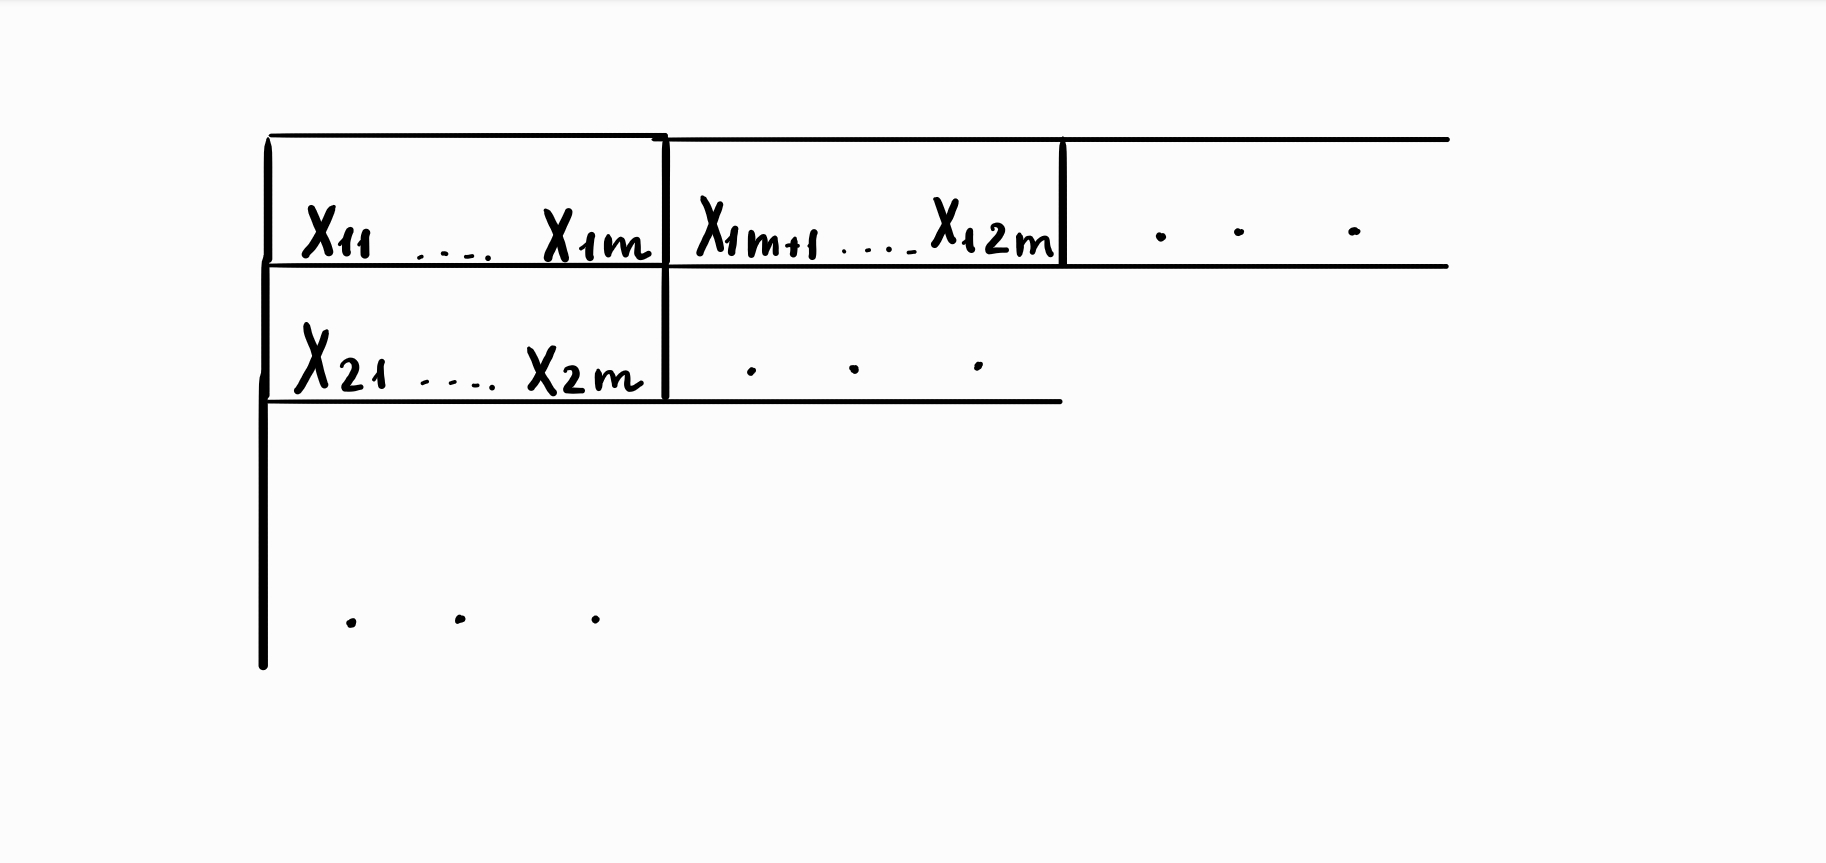
\includegraphics[width=0.7\linewidth]{Кодировка для SAT.png}
    \end{figure}
    \noindent Теперь по этим переменным будем писать формулу: предположим, что $q_0 = 10011$. Строим $\varphi$: \[\varphi = (x_{11} \equiv 1) \wedge 
    (x_{12} \equiv 0) \wedge (x_{13} \equiv 0) \dots \wedge ( * ) \wedge (\square) \wedge (\lhd) \wedge (**) \label{eq:2} \tag{2}\]
    \[ * \text{ --- посимвольная проверка того, что здесь находится } x\] \[** \text{ --- проверка перехода с 1 строки на 2}\] 
    Проверка перехода на другую строку --- это фактически проверка красной доминошки некоторой сложной громоздкой формулой, которая, тем не менее,
    является константной. Заметим, что проверку сертификата мы не делаем (потому что мы и не знаем, какой сертификат нам нужен). Также мы выбираем такой
    верификатор, что он стирает все с ленты, записывает на нее $1$ и останавливается в состоянии $q_a$, если сертификат является выполняющим набором.
    Продолжаем строить формулу:
    \[\varphi = (\ref{eq:2}) \wedge (\text{переход с 2 на 3}) \wedge \dots \wedge (\rhd q_a 1 \# \dots \#\lhd)\]
    Заметим, что нам не нужно отслеживать, одно ли у нас состояние в каждой строке, потому что верификатор является ДМТ, и никакой неопределённости 
    быть не может. \\ Итак, мы получили очень большую страшную формулу, при этом она выполнима $\Longleftrightarrow$ протокол корректен, то есть,
    корректен сертификат, и верификатор на этом сертификате останавливается в принимающем состоянии. Такими вот движениями мы доказали, что произвольный 
    язык $L \in \NP$ полиномиально сводится к $\SAT$. Пару слов о полиномиальности: квадратичную таблицу от $P(|x|)$ мы завели за полином, построили формулу 
    тоже за полином (тоже что-то около квадрата).
\end{proof}

\begin{theorem}
     \[\tSAT \in \NPC\]
\end{theorem}

\begin{proof}
    Для доказательство нужно свести $\SAT \leq_p \tSAT$ (обратная сводимость очевидна, потому что $\tSAT$ --- частный случай $\SAT$. К тому же,
    $\tSAT \in \NP$ опять-таки в силу того, что $\tSAT \subset \SAT$ и $\SAT \in \NP$). Пусть у нас есть 
    страшная формула, например \[\varphi = \left((x \equiv y) \to (\lnot z)\right) \oplus ((\lnot x) \to z)\] Нарисуем дерево этой формулы:
    \begin{figure}[H]
        \centering
        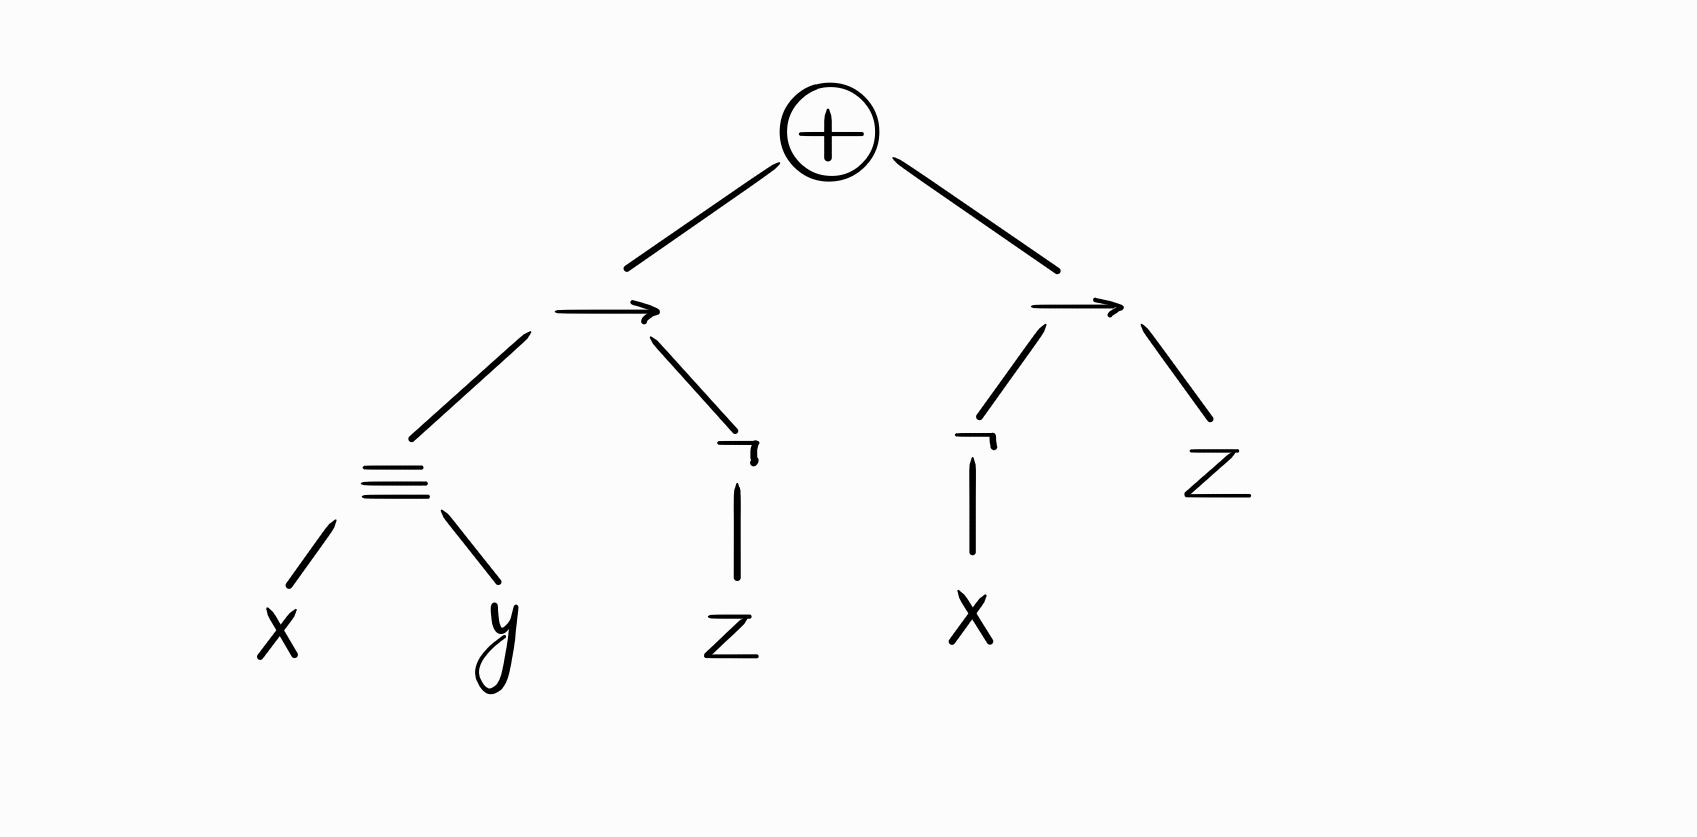
\includegraphics[width=0.6\linewidth]{Дерево формулы.png}
    \end{figure}
    \noindent Заметим, что каждый символ в формуле, кроме скобок, присутствует в дереве только 1 раз. Значит, у нашей формулы не более чем линейно подформул
    (каждой подформуле соответствует ветка (поддерево данной вершины), а количество веток равно количеству вершин). Теперь на каждую подформулу, кроме 
    листов, заведём отдельную переменную и будем превращать исходную формулу в 3-КНФ следующим образом: каждой вершине $a$, имеющей детей $b$ и $c$
    будем сопоставлять формулу вида \[a \equiv (b \ op \ c)\] А любая такая формула имеет своё 3-КНФ представление, причем в этом представлении не более 8
    дизъюнктов. Все такие формулы мы будем объединять через конъюнкции, причём таких конъюнкций наберётся не более, чем линия по длине формулы (потому что
    у каждой вершины дерева не более чем 8 дизъюнктов по 3 переменные). И не забудем потребовать, чтобы переменная, соответствующая корню дерева, равнялась 1.
    \\ Таким образом, мы построили всюду определённую полиномиально вычислимую функцию,
    которая по произвольной формуле $\varphi$ строит формулу $\varphi'$ в виде 3-КНФ, и $\varphi$ выполнима $\Longleftrightarrow \varphi'$ выполнима.
    То есть, мы свели $\SAT$ к $\tSAT \Longrightarrow \tSAT \in \NPC$. 
\end{proof}
\end{document}